%!TEX root = ../report.tex

% 
% Related work
% 

\section{Related Work (17pgs)}
\label{sec:rw}

%%%
\subsection{General-purpose systems}

The systems in this category are built to support all, or at least substantial part, of the software development process. For this purpose, they suggest an \ac{ide} that aims to support the entire process by grouping in a single environment all necessary tools. The tools are minimal modules of functionality which can be implemented and delivered separately. Consequently, the designers of these systems focus on trying to create programming tools that allow people to build as much as possible.

In this section we describe in the detail the systems whose main features are primary contribution. Which means that we select two representative systems among those which provides common features. The first is Eclipse~\cite{carlson2005eclipse} between NetBeans~\cite{boudreau2002netbeans}, IntelliJ~\cite{intellij2001intellij} and Microsoft Visual Studio (MVS)~\cite{guckenheimer2006software}. And the second is LightTable\footnote{\label{lt:note}\texttt{http://lighttable.com/}} between Xcode\footnote{\texttt{https://developer.apple.com/xcode/}}.
%%%%%%%%%%%%%%%%%%%%%%%%%%%%%%%%%%%%%%%%%%%%%%%%%%%%%%%%%%%%%%%%%%%%%%%%%%%%%%%%%%%%%%%%%%%%%%%%%%%%%%%%%
\subsubsection{Eclipse~\cite{carlson2005eclipse}} is a popular \ac{ide} used mainly by Java developers, although it supports other programming languages such as C, C++ and JavaScript. Commonly cited reasons for using Eclipse include rich Java development tools support and a \texttt{plugin} architecture, the Eclipse Platform~\cite{DesRivieres2004}, that allows tight integration of third-party functionality.

The Eclipse platform~\cite{DesRivieres2004} has a common architecture among the \ac{ide}s studied in this report. This architecture is characterized by two main components. The \textit{plugin}, the smallest unit of function that can be developed and delivered separately. And the platform runtime, the component which will discover and connect the \textit{plugins} to the platform itself. As a result, the platform offers interoperability between several tools that are used in distinct phases of the software development process.

Eclipse provides many other features. We are particularly interested on those which works as the programmer codes, to provide feedback to the programmer. These includes syntax highlighting, code completion suggestions, and indications of problems associated with various locations in a source file. These features minimize the effort to write syntactically correct code and minimize the latency until the code written can be executed. Facilities for editing running code also exist, due to the new capability of the \ac{jvm}, from version 1.4. It has included a swap feature that enables the replacement of a class file by a new one while the overall program is running. That permits \ac{ide}s to offer a code push feature to quickly compile a new version of a class and/or object and insert it into the running \ac{jvm}.

In general, Eclipse including the other \ac{ide}s, which provide common features, also share the following common drawbacks:
\begin{itemize}
	\item They are incidentally complex. This means that there are immense amount of work to be done that is not directly related to the real problem itself. For instance, until the programmer get a simple program to run, he needs to install and configure, in his development machine, all set of necessary software. That is a tiresome task, for the most programmers.
	\item Programming in those \ac{ide}s are unobservable. This means that the only way to see how the program executes is by a stepwise debugger, which forces the programmer to stop the program and look at a single instant in time. So he cannot see, at glance, how his program execute. Nor how his changes affect his program. And nor how his programs are connected together.
\end{itemize}
%%%%%%%%%%%%%%%%%%%%%%%%%%%%%%%%%%%%%%%%%%%%%%%%%%%%%%%%%%%%%%%%%%%%%%%%%%%%%%%%%%%%%%%%%%%%%%%%%%%%%%%%%
\subsubsection{LightTable\protect\footnotemark[\ref{lt:note}]} is a programming environment which aims to turn programming in something more observable. Bret Victor, in his influential work~\cite{inventingPrin,learnableProg}, pointed out serious problems with programming nowadays and showed, with some prototypes, how the environment can address those problems. Base on those ideas, LighTable was implemented and its features represent the state of art. It is commonly used by professional programmers to build web applications. There are, at least, two features which helps in this process. First, live execution feedback were the code is executed instantly and the program's flow showed at right panel. And second, the organization of code in tables enabling quick access.

LightTable was initially written in Clojure (a dialect of Lisp, which compiles directly to JVM bytecode) and actually has moved, almost the entire implementation, to ClojureScript (a Clojure compiler that targets JavaScript). The reason behind this decision seems to be because in an web application the effort for changing and prototyping be smaller. Consequently, adding new UI or change the existing ones in LightTable is doable while in Eclipse, for instance, would require few weeks. Moreover, ClojureScript's programming model, besides to share with Lisp the philosophy code-as-data, it provides the macro machinery on top of JavaScript.

The program documentation in LightTable are always available. When the programmer move the cursor over a function identifier, the available function's documentation is displayed at right panel. This feature is useful, because it enables the reader to effortless read the program. Then, he can concentrate in what is really genuine. However, it just relates the predefined functions with the existing documentation. The problem of understanding the genuine functions yet remains. 

\begin{wrapfigure}{r}{0.3\textwidth}
  \vspace{-25pt}
  \begin{center}
    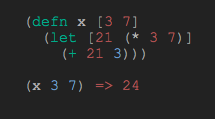
\includegraphics[width=0.3\textwidth]{img/eval-close}
  \end{center}
  \vspace{-20pt}
 \caption{LightTable real-time debugger.}  
  \vspace{-20pt}
    \label{fig:lt2}
\end{wrapfigure}

On the other hand, programmers are encouraged to understand functions by seeing how values of a function call flow thought it. That is no more than improving the old idea of lispers environment where we can try out expressions in a REPL. However it uses reflection mechanisms to trace the values of function call and shows how the code is filled in. For example, if the programmer defines a function \texttt{x} in the editor and then calls it with \texttt{(x 3 7)}. In right panel will appear the same function definition filled with the called values, as showed in Figure~\ref{fig:lt2}. 

The real-timer debugger represents an interactive way to debug code by understanding the program flow. However using this feature in a complex groups of functions is worthless. Because, all the programmer sees is a replica of his functions filled with numbers. A poor representation of the flow which forces the programmer to spend as much effort with this feature as without it. For this reason others systems, described in this report, represent the program flow using arrows which seems to be more appropriate.

Despite of being a state of art programming environment, LightTable remains on a experimental phase. It is not robust as the presented popular IDEs.
%%%%%%%%%%%%%%%%%%%%%%%%%%%%%%%%%%%%%%%%%%%%%%%%%%%%%%%%%%%%%%%%%%%%%%%%%%%%%%%%%%%%%%%%%%%%%%%%%%%%%%%%%
\subsection{Teaching systems}

Unlike the previous systems, these systems are designed with the goal of helping people learn to program. Most of the systems in this category provide simple programming tools that exposure the novice programmers to some of the fundamental aspects of the programming process. After gaining experience with a teaching system, students are expected to move to more general-purpose environment. 

%%%%%%%%%%%%%%%%%%%%%%%%%%%%%%%%%%%%%%%%%%%%%%%%%%%%%%%%%%%%%%%%%%%%%%%%%%%%%%%%%%%%%%%%%%%%%%%%%%%%%%%%%
\subsubsection{LOGO~\cite{papert1980mindstorms}} is a programming language and environment intended to allow children to explore a wide variety of topics such as physics and mathematics. The programming language is a dialect of Lisp with much of the punctuation removed to make the syntax accessible to children. Indeed the most notorious LOGO's innovation was in the metaphor that the programming language represent.

\begin{wrapfigure}{r}{0.35\textwidth}
  \vspace{-25pt}
  \begin{center}
    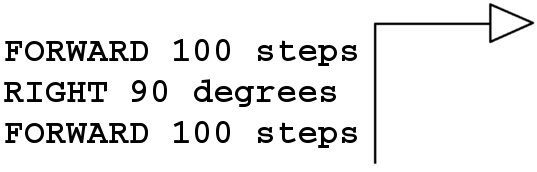
\includegraphics[width=0.35\textwidth]{img/turtle}
  \end{center}
  \vspace{-20pt}
 \caption{Directing the ``turtle''.}  
  \vspace{-20pt}
    \label{fig:turtle}
\end{wrapfigure}

In Logo, the programmer draws pictures by directing the ``turtle'', an onscreen character which leaves a trail as it moves. The turtle serves a number of functions, but the most important is that the programmer can identify with it. To figure out how to make the turtle perform an action, the programmer can ask how he would perform that action himself, if he were the turtle.

For example, to figure out how to draw a circle, a learner will walk around in circles for a bit, and quickly derive a ``circle procedure'' of taking a step forward, turning a bit, taking a step forward, turning a bit. After teaching it to himself, the learner can then teach it to the computer. The turtle is the in-computer embodiment of the programmer himself, a self, like the player-character in a video game, and thereby allows the learner to 
transfer his knowledge of his own body into knowledge of programming.

LOGO has influenced several systems, and its principles show how a system can be designed around the way people think and learn.
%%%%%%%%%%%%%%%%%%%%%%%%%%%%%%%%%%%%%%%%%%%%%%%%%%%%%%%%%%%%%%%%%%%%%%%%%%%%%%%%%%%%%%%%%%%%%%%%%%%%%%%%%
\subsubsection{SmallTalk~\cite{Kay1993}} is a programming language and environment to support children in the world of information. The designers of this system, wanted to create a programming language with a simple model of execution and a method of programming that could accommodate a wide variety of programming styles. Small talk was based around three ideas: (1) everything is an object, (2) objects have memory in the form of other objects, (3) and objects can communicate with each other through messages.

Like LOGO, the communication through messages has a strong resonant metaphor. To program the behavior of an object, the programmer casts himself into the role of that object (to the extent of referring to the object as ``self'') and thinks of himself as carrying on a conversation with other objects. This is a powerful metaphor, because role-playing and conversing are powerful innate human facilities. 
%%%%%%%%%%%%%%%%%%%%%%%%%%%%%%%%%%%%%%%%%%%%%%%%%%%%%%%%%%%%%%%%%%%%%%%%%%%%%%%%%%%%%%%%%%%%%%%%%%%%%%%%%
\subsubsection{Processing~\cite{Reas2006}} is a programming language and environment designed to teach programming aided by a visual context. It has become popular among students, artists, designers, architects, and researchers. Processing acts as a tool to get non-programmers started with programming through the instant visual feedback. As a result, a new programming language and environment were tailored around this purpose.

The programming language is built on top of Java, it removes the much of the verbosity of Java to make the syntax accessible to novices. The language provides simple access to external libraries such as OpenGL, through single entry points, such as \texttt{setup} and \texttt{draw}. This allows novices to quickly prototype and learn fundamental concepts of programming and eventually learn other languages.

The programming environment contains a simple text editor, a text console to present errors and a run button. The run button compiles the Processing code and execute it. In the default mode, the result is presented in a 2D graphical window. However the render can be configured to present the result in 3D and also recurring directly to the graphics broad using shader. And actually, the Processing code can be exported, with few changes, as an application for different platforms such as Java, JavaScript and Android. For example, to export for JavaScript is just necessary to create a new HTML page and include the Processing code as an script. The Processing code will be translated to JavaScript and will use as the render the new capabilities of the HMTL5 canvas with WebGL.

The popularity of Processing can be explained by these features besides of being a domain-specific language. However Processing present the following relevant issues which could discourage the learning: (1) Weak metaphor. In Processing, by contrast with the previous system, the programmer has no identity within the system. There are no strong metaphors that allow the programmer to translate his experiences as a person into programming knowledge. (2) Decomposition. Processing does not encourage the fundamental approach to solve a complex problem by breaking it into simpler problems. Because drawing and input events are tied to single entry points. The behavior of submodules must be tangled across these global functions. Clean decomposition is not possible. (3) Recomposition. Processing does not encourage combining two programs. The programmer can not just grab and use part of other programs, variables must be renamed or manually encapsulated; the \texttt{draw} and mouse functions must be woven together, and so on. Even worst Processing has global modes which alter the meaning of function arguments. For example, two Processing programs can specify its colors in different modes and each mode has its proper meaning of \texttt{fill} function arguments. Combining those programs will be almost hopeless. (4) Readability. The syntax of a Processing program represent a significant barrier for reading. For example the function which draws an ellipse on screen is written as \texttt{ellipse(50,50,100,100)}. The reader must lookup or memorize every argument. (5) Environment. The programming environment is fragile, it does not attempt to solve any of the previous issues related with the language and its implementation. 
%%%%%%%%%%%%%%%%%%%%%%%%%%%%%%%%%%%%%%%%%%%%%%%%%%%%%%%%%%%%%%%%%%%%%%%%%%%%%%%%%%%%%%%%%%%%%%%%%%%%%%%%%
\subsubsection{Fluxus\protect\footnote{\texttt{http://www.pawfal.org/fluxus/}}} is a programming language and learning environment designed for rapid prototype using 3D graphics and sounds. This emphasis on rapid prototype and quick feedback make Fluxus a tool for learning computer animation, graphics and programming. However, the most users of Fluxus use it for livecoding; the act of performing coding lively to an
audience.

Fluxus is mainly written in C++ and it is statically linked to several shared libraries, specified at compile time. For instance, Fluxus uses \texttt{jack-audio, ode, fftw} to handle and synchronize the audio, \texttt{GLEW} to present graphics and \texttt{racket3m} to embed the Racket run-time system into the application. So, the Fluxus programming language is an extension of Racket (a descendant of Scheme) with graphical commands. 

Like Processing, Fluxus provides simple access to those libraries through single entry points, for instance \texttt{start-audio} connects an input audio to the application, \texttt{every-frame} register a function called once per frame, and so on. However, it represents an barrier for decomposition since the behavior of submodules must be tangled across these global functions.

Fluxus has its own environment, tailored for livecoding. It is composed by a graphical window with a simple text editor. The programmer types his code on the editor and press a shortcut key each time he wants to run the code. Fluxus evaluates this code through Racket run-time system and shows its result in the same graphical window that the code was written. This mechanism is valuable in an livecoding environment, because the performer can be editing the code while the result of the previous computation is maintained at background. On other hand, if the code has any errors and the performer execute it, the previous computation disappears and the environment will not help to find it. This is a serious problem, specially when it is the syntax of Racket.

Moreover, Fluxus share with Processing the similar drawbacks previously stated. However Fluxus can be used as a module of DrRacket programming environment. The above problem and many others were solved in DrRacket.
%%%%%%%%%%%%%%%%%%%%%%%%%%%%%%%%%%%%%%%%%%%%%%%%%%%%%%%%%%%%%%%%%%%%%%%%%%%%%%%%%%%%%%%%%%%%%%%%%%%%%%%%%
\subsubsection{DrRacket~\cite{findler2002drscheme}} is a programming environment designed to overcome problems related with the Racket language and its implementation. DrRacket is one of few programming environments which supports gradual learning in a more general language from the start. Consequently, it has been widely used in introductory programming courses for several universities around the world.

The common case where DrRacket is used is to teach functional programming, namely Racket. To facilitate this process DrRacket contains three tools. The first is a symbolic stepper. It models the execution of Racket programs as algebraic reductions, since Racket is implemented on top of lambda calculus. The second tool is a syntax checker. It annotates programs with font and colour changes based on the syntactic structure of the program. It also permits students to explore the lexical structure of their programs graphically and to $\alpha$-rename identifiers. The third tool is a static debugger that infers what set of values an expression may produce and how values flow from position to position in the source text. And, upon demand, it explains the reason of errors by drawing value flow graphs over the program text.

DrRacket also share with lisp environments the read-eval-print loop (REPL). A command prompt intended to quickly execute expressions and print its output. Specially in a learning environments this feature makes an important connection between program execution and algebraic expression evaluation. However the Lisp-style syntax obscured the effect of this feature. To overcome this limitation, DrRacket provides a \texttt{pretty-printer}. A module capable of printing algebraic expressions in a meaningful way, as well as other graphics elements supported by the text editor such as images, snips, XML boxes, and so on.

From the perspective of professional programmers DrRacker can be a potential target. It is useful for the development of complex applications, including the DrRacket itself. Moreover it is extensible by the same API which actually the above tools implement. Through this API is even possible to extend the REPL, as in Pict3D\footnote{\texttt{https://github.com/ntoronto/pict3d}} (a 3D engine that integrates new graphical elements in the DrRacket environment). On other hand, to support this kind of extensions, among others, DrRacket's architecture has become increasingly complex. For instance to make a simple change in a editor's element the programmer should be able to understand several modules, unrelated with the problem itself. This extra complexity is perhaps a strong reason to not choose DrRacket as a basis to develop tools.

Moreover, DrRacket seem to need new mechanism which facilitates novices to read code and to execute it. The racket syntax represent a barrier for learning. But these problems can be mitigated with specific features.
%%%%%%%%%%%%%%%%%%%%%%%%%%%%%%%%%%%%%%%%%%%%%%%%%%%%%%%%%%%%%%%%%%%%%%%%%%%%%%%%%%%%%%%%%%%%%%%%%%%%%%%%%
\subsubsection{PythonTutor~\cite{GuoSIGCSE2013}} is a web-based program visualization tool, designed to explain how a piece of Python code executes. It has become popular among students from introductory Computer Science courses. Using this tool, teachers and students can write Python programs directly in the web browser and navigate step by step throughout execution to view the run-time state of data structures. The global variables and stack frames at the current execution point to visual representations of Python objects. For example, a global variable that defines a tuple will be represented with a arrow that point to a box with two divisions.

PyhtonTutor has two main modules: the backend which implements the tool core functionality and the frontend which presents the program's visualization. The backend executes the input program under supervision of the standard Python debugger module (\texttt{bdb}), which stops execution after every executed line and records the program's run-time state. After execution terminates, the backend encodes the trace in JSON format, serializing Python data types into native JSON types with extra metadata tags and send it to the frontend. The frontend renders the objects using standard web technologies: HTML, CSS, and JavaScript. In this way, users can use the tool without installing any extensions or plugins.

A major concern in PythonTutor is the security, because the PythonTutor's backend executes untrusted Python code from the web. To prevent the execution of dangerous constructs such as {\tt eval}, {\tt exec} and {\tt file I/O}, PythonTutor implements sandboxing. Basically, it denies the use of most module imports, by parsing the user's code importing. A strict approach, but effective in this case.

The PythonTutor tool allows the programmer to follow the program's execution over time. But, the programmer is seeing a single point in time at any instant. There is no visual context. The entire flow is represented by disconnected points in time. For example, the programmers who wants to understand a conditional algorithm, using this tool will not see the pattern of the algorithm neither understand it at a higher level.
%%%%%%%%%%%%%%%%%%%%%%%%%%%%%%%%%%%%%%%%%%%%%%%%%%%%%%%%%%%%%%%%%%%%%%%%%%%%%%%%%%%%%%%%%%%%%%%%%%%%%%%%%
\subsubsection{YinYang~\cite{mcdirmid2013usable}} is a prototype of a programming language and environment whose main feature is the live execution feedback. That means it combines editing and debugging, where updated debug results are conveniently visible while editing. YingYang addresses the above issue in two ways. First, as well as the previous system, it allows programmers to see single points of execution directly within the code editor (probe; precede expressions with \texttt{@} operator). Second, it has a pane aside the editor which traces execution with entries that are navigable (trace; print-like statements). Basically, the trace is a enhanced display function which combined with ``probes'' allows the state of previous executions be restored. So, programmers can take in the entire program's flow at a glance and navigate trough it using probes.

YingYang uses an incremental framework as basis of its programming model. This framework decomposes the program execution into a tree of nodes that can be re-executed independently on a code or input change. However, it cannot be performed transparently. It requires programmers to specify how the program will be decomposed. So programmers must deeply understand the granularity and modularity characteristics of the computations being performed by the program. Otherwise changes can sometimes have a huge impact on program re-execution time ($\sim$50ms). So live programming would actually reduce programmer productivity as programmers depend on but wait for slow feedback.

Although YinYang provides usable features for a learning environment, such as allowing learners to navigate through the program execution, it does not have a suitable language. The language has no metaphor, and to use the features the programmers must include trash in the code. 

%%%%%%%%%%%%%%%%%%%%%%%%%%%%%%%%%%%%%%%%%%%%%%%%%%%%%%%%%%%%%%%%%%%%%%%%%%%%%%%%%%%%%%%%%%%%%%%%%%%%%%%%%
%%%
\subsection{Empowering Systems}

The systems in this category are built with the belief that the important aspect of programming is that it allows people to build things that are tailored to their own needs. Consequently, we describe in this section how systems from two distinct areas are being tailored to achieve their user's needs. First, in Architecture where new programming languages and environments are being proposed to support the increasing use of \ac{gd}; a design method that uses algorithms to generate architectural models, usually in a \ac{cad}. Second, in Mathematics with the well known plots and graphics. 

%%%%%%%%%%%%%%%%%%%%%%%%%%%%%%%%%%%%%%%%%%%%%%%%%%%%%%%%%%%%%%%%%%%%%%%%%%%%%%%%%%%%%%%%%%%%%%%%%%%%%%%%%
\subsubsection{DesignScript~\cite{aish2012designscript}} is a programming language and environment designed to support \ac{gd} with textual methods. It is mainly used by architects and designers to generate geometric models for AutoCAD. Instead of creating geometric models manually by manipulating UI icons, designers can automate this process with a script. When the script is executed a geometric model is generated in the AutoCAD. The Figure~\ref{fig:ds} shows five spheres being created using a script.

\begin{figure}[!htbp]
  \centering
  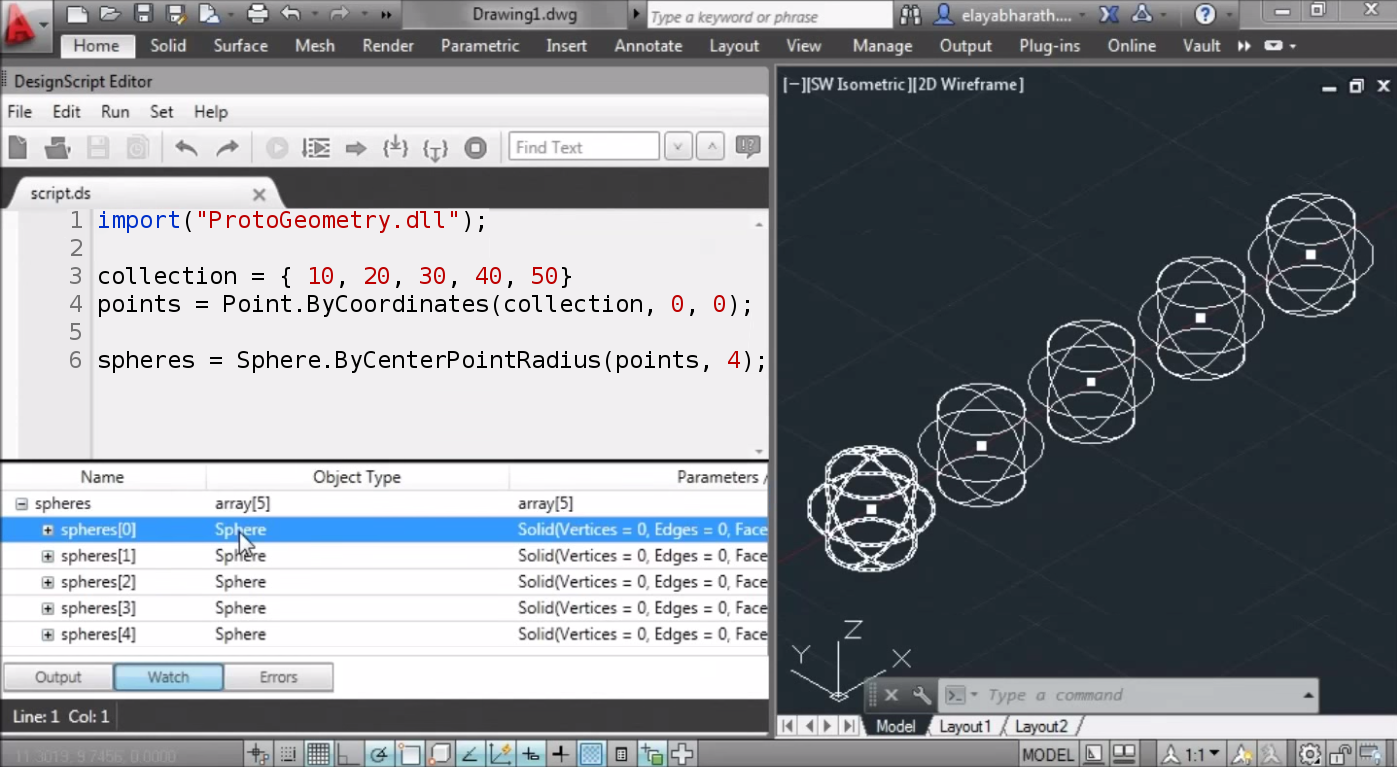
\includegraphics[width=1.0\textwidth]{img/designScriptIDE}
    \caption{DesignScript programming environment.}  
  \label{fig:ds}
\end{figure} 


\begin{wrapfigure}{r}{0.4\textwidth}
  \vspace{-25pt}
  \begin{center}
    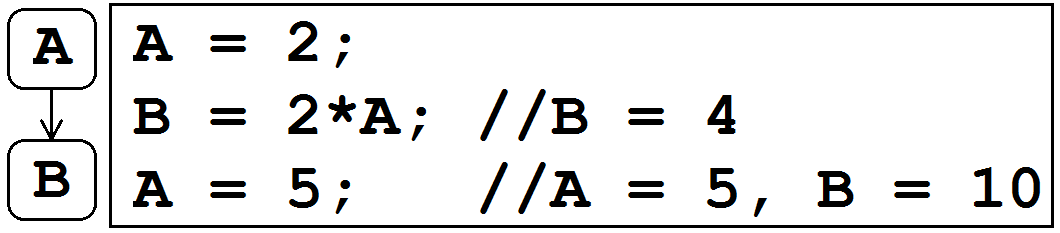
\includegraphics[width=0.4\textwidth]{img/designscript}
  \end{center}
  \vspace{-20pt}
 \caption{Associative interpretation.}  
  \vspace{-20pt}
    \label{fig:designscript}
\end{wrapfigure}

The programming language is presented as an associative language. The variables are abstract types that can represent numeric values or geometric entities. These variables are maintained in a graph of dependencies. When a change in a variable occurs it forces the re-evaluation of the graph, as showed in Figure~\ref{fig:designscript}. Consequently a subsequent change to a variable has impact on its previous use. This feature is useful, specially in a modeling environment, because allows the geometric entities be changed giving continuous feedback to the designer.

The DesignScript's programming environment provides a text editor coupled into AutoCAD, an interpreter, a simple debugger and few tabs on the bottom. The language interpreter is invoked each time that the designer clicks on the run button. Then all the script is interpreted and its result produces geometric entities rendered in the CAD. The continuous feedback feature just work in debug mode, because in this mode the script is interpreted line by line. So each set to a variable will change its dependencies and will recompute the model. However, in debug mode the code cannot be edited. Consequently, this feature is worthless during code editing.

In the DesignScript's debug mode users can inspect the values of variables by adding watchers to them. So the values of those variables are showed in the watch tab. If the contents of a variable represent a geometric model then the respective model in the CAD is highlighted. For example in the Figure~\ref{fig:ds}, the \texttt{spheres} variable is being inspected and its first value was selected. However the inverse, highlighting a model in the CAD and show the variable in the code, is not supported.

A typical mechanism of live programming environments such as sliders are also supported by the DesignScript's environment. The sliders are supposed to be used by quickly experiment new values. So designers can create new models reacting by the changes. However, in the DesignScript's sliders the changes just reflect in the models when the designer drops the slider. Until there the designer should imagine how would be the model with the dragged value. It is completely against the purpose of the sliders.

Moreover the DesignScript language, despite of being presented as pedagogic, has some drawbacks. It does not carries any strong metaphor which helps beginners to start with the language. Additionally the associative paradigm represents an barrier for sharing code. Because it discourages the recomposition of modules, since new modules can change the previous one. The environment provides poor mechanism that help people to find bugs in the code. Finally, a DesignScript is confined to only produce geometry to AutoCAD.
%%%%%%%%%%%%%%%%%%%%%%%%%%%%%%%%%%%%%%%%%%%%%%%%%%%%%%%%%%%%%%%%%%%%%%%%%%%%%%%%%%%%%%%%%%%%%%%%%%%%%%%%%
\subsubsection{Monkey\protect\footnote{\texttt{http://wiki.mcneel.com/developer/monkeyforrhino4}}} is a programming environment designed to support \ac{gd} with textual methods. Like DesignScript Monkey is used to edit, debug and interpreter scripts. However Monkey uses DesignScript as its programming language and Rhinoceros3D\footnote{\label{rhin}\texttt{https://www.rhino3d.com}} (or Rhino for short), a lighter \ac{cad} than the AutoCAD, to generate the geometric models.

Monkey is implemented as a plugin for Rhino4. It uses a \texttt{.NET} frame work to communicate with the \ac{cad}. So the scripts are written outside of the \ac{cad}'s environment and upon execution the plugin, through the frame work, invokes the \ac{cad} primitives to generate the models. It has an advantage, relatively the previous system, because it is \ac{cad} independent. On the other hand, it depends on the frame work which must exist in the user's machine.

In fact, Monkey is pretty based on general-purpose environments. It provides typical features of those environments, namely syntax highlighting, auto-completion and error highlighting. And even the organization of code into trees are similar. However, this influence seems awkward when the community that will use these tools are mostly composed by beginners in programming. Moreover, similar to DesignScript, the RhinoScript just produce geometry to Rhino4. Consequently Monkey is \ac{cad} dependent. 
%%%%%%%%%%%%%%%%%%%%%%%%%%%%%%%%%%%%%%%%%%%%%%%%%%%%%%%%%%%%%%%%%%%%%%%%%%%%%%%%%%%%%%%%%%%%%%%%%%%%%%%%%
\subsubsection{Rosetta~\cite{lopes2011portable}} is a programming environment designed to support \ac{gd} with textual methods. Like Monkey, Rosetta provides its own environment detached from the \ac{cad}. Rosetta is a step forward from the previous systems, because it solves the portability problem among \ac{cad}s. In Rosetta a \ac{gd} program can be written in various programming languages (frontends) and the geometric models can be rendered by various \ac{cad}s (backends). As a result, designers are free to write their programs in their preferred frontend which, upon execution, will generate the same geometry for the various backends. In Figure~\ref{fig:rosetta}, a program is written in Racket and its execution produces geometry for AutoCAD.

\begin{figure}[!htbp]
  \centering
  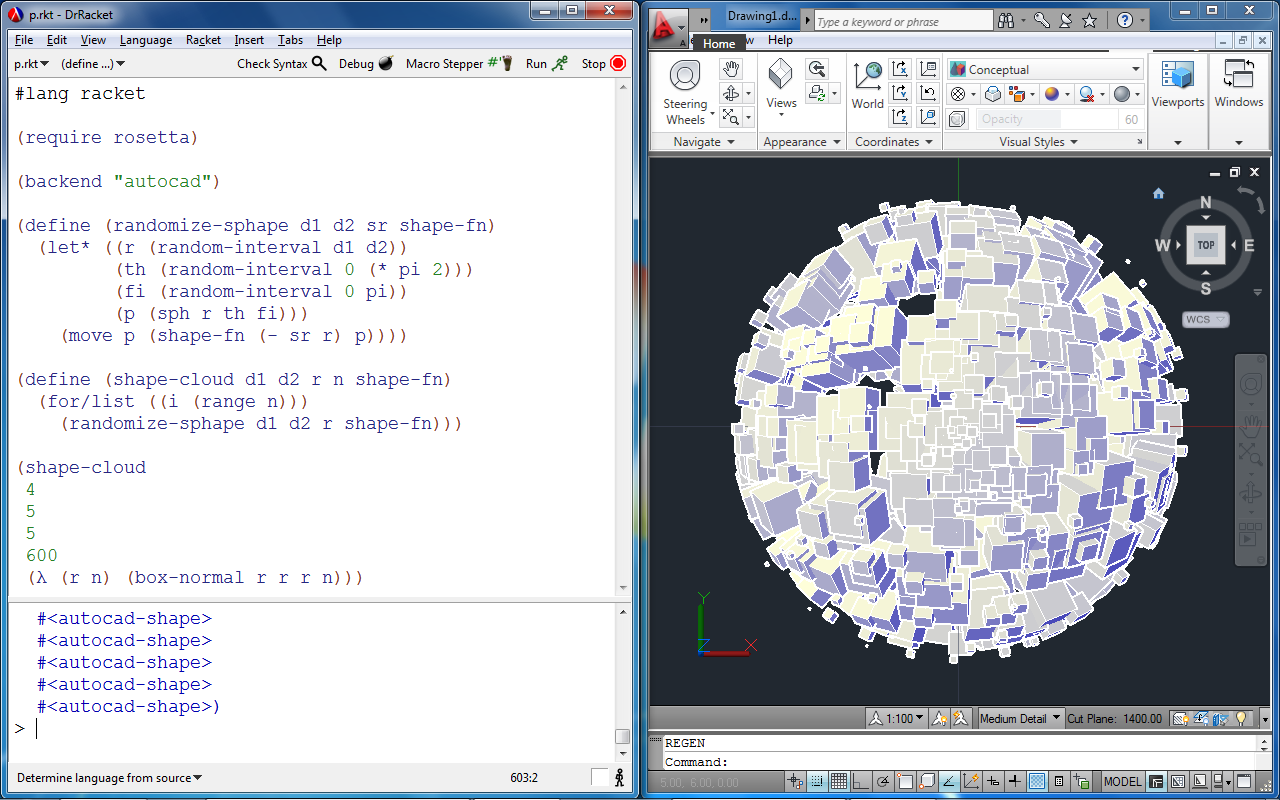
\includegraphics[width=1.0\textwidth]{img/rosetta1}
    \caption{Rosetta programming environment.}  
  \label{fig:rosetta}
\end{figure} 

Rosetta has been used to teach programming in an architecture course. Tailored to this end, Rosetta uses DrRacket~\cite{findler2002drscheme} as its own programming environment. The DrRacket environment serves a number of functions, but the most important is that the student can start immediately to learn programming. For instance, the environment is set up with just three lines of code. As shows Figure~\ref{fig:rosetta}, the \texttt{\#lang} specifies the frontend language, the \texttt{require} imports Rosetta's primitives and finally the \texttt{backend} names a possible backend.

The Racket language is also an advantage of Rosetta's environment. Because, mainly, it encourages the development of the mathematical paradigm for writing algorithms. In this way, students that learn simple programming techniques, such as recursion, are able to create robust models. And as the students progress new programming languages are also available to learn, such as JavaScript, Python, Processing and so on.

The Rosetta's environment present some interesting tools for \ac{gd}. A programming flow tracer, similar to the DesignScript's watcher, that allows the designer to select a function call and see the respective generated object highlighted, in the \ac{cad}. This feature goes further than the DesignerScript's watcher by allowing the inverse. Highlighting a model in the CAD will show in DrRacket's editor a path of functions call which produced that object. And an interactive slider tool proposed as an attempt to provide immediate feedback to the designers. The slider's callback is the function whose produces the entire model, so each time the slider change this function will be called. Consequently a new model will be generated.

Undoubtedly Rosetta's environment goes further than the textual environments for \ac{gd} presented in this report. However it presents some drawbacks which may discourage the learning in general. Beginning with the usual programming language: Racket. The syntax of Racket program represent a significant barrier for reading. For instance the function which draws a circle in the \ac{cad} is written as \texttt{(circle (xy 0 0) 1)}. The reader must lookup or memorize every argument. Using the Rosetta's documentation the reader will spend even more time, because it is in a book mixed with architecture subjects. Moreover, the immediate feedback confines to re-execute the same function with different arguments.
%%%%%%%%%%%%%%%%%%%%%%%%%%%%%%%%%%%%%%%%%%%%%%%%%%%%%%%%%%%%%%%%%%%%%%%%%%%%%%%%%%%%%%%%%%%%%%%%%%%%%%%%%
\subsubsection{Grasshopper\protect\footnote{\texttt{http://www.grasshopper3d.com/}}} is a programming language and environment designed to support \ac{gd} with visual methods. Grasshopper provides an alternative way to programming. By definition, it is a bi-dimensional representation consisting of iconic components that can be interactively manipulated by the user according to some spatial grammar~\cite{myers1990taxonomies}. For example, the boxes in Figure~\ref{fig:grass} are components which receive the input (left ports) perform some operations and return the output (right port). The components are linked to other components establishing a \textit{dataflow} paradigm where the input of a component is the output of another.

\begin{figure}[!htbp]
  \centering
  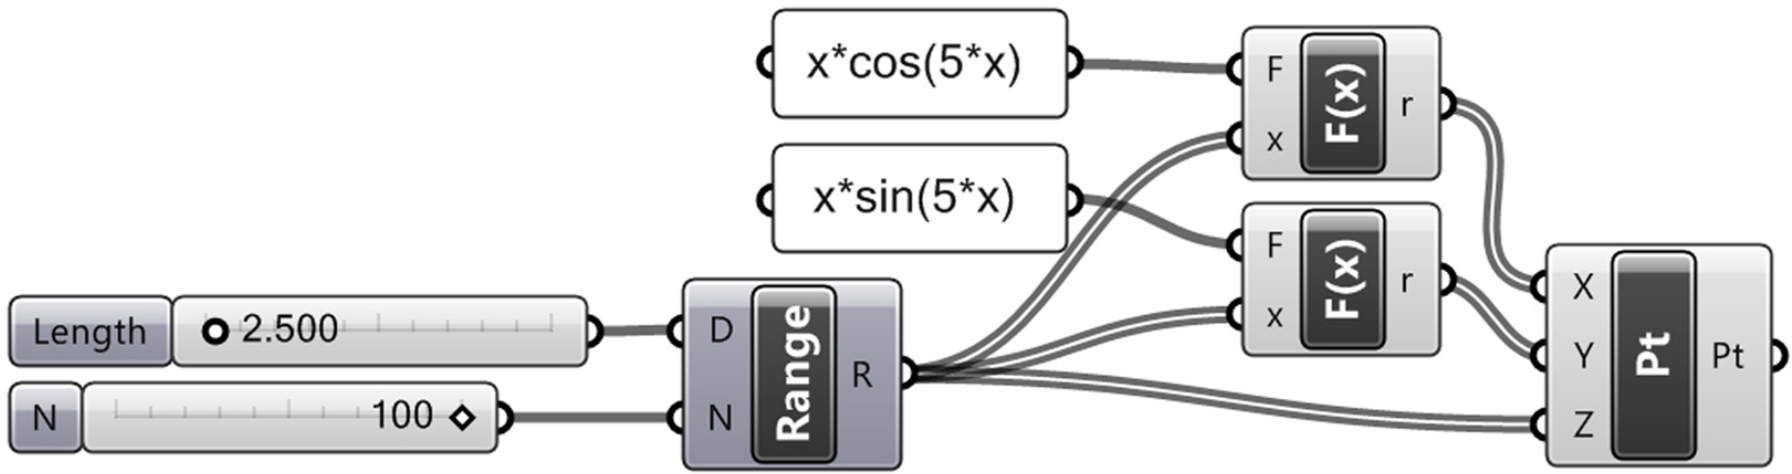
\includegraphics[width=0.8\textwidth]{img/grasshopper}
    \caption{A program in Grasshopper that computes the 3D coordinates of a conical spiral. Each time the left sliders are dragged a new coordinate is calculated.}
  \label{fig:grass}
\end{figure}

Like Monkey, Grasshopper is implemented as a \textit{plugin} for Rhino\footnotemark[\ref{rhin}]. However Grasshopper tailors the Rhino's environment with specific \ac{gd} tools. These tools are the state of art, because they implement important principles for design models, such as the following:

\begin{itemize}
 \item \textit{Get immediate feedback}. As the user interacts with the components, by adding and connecting them, the result reflects immediately in the \ac{cad} model. It facilitates the design conception, because the user's intentions are immediately visible. 
 \item \textit{Facilitate program input}. To facilitate the process of design exploration, Grasshopper provides sliders which are connected at the components' input. Dragging the slider causes a change propagation through components. The components are re-executed with the new slider's value. Combined with the above feature new models are generated immediately.
 \item \textit{Correlate the program with generated elements}. Like DesignScript's watcher, by selecting a component its geometry is highlighted in the \ac{cad}. It allows designers to better understand a program by figuring out the roles of each component.
 \item \textit{Show comparisons between models}. Grasshopper provides a special component that, when connected at the output of another component, replicates the geometry. This mechanism is useful for design exploration, because it maintains in the \ac{cad}'s background an old replica of the changed geometry. It adds a context at each change, so the designer can compare the result of his change in the new geometry based on the old one.
\end{itemize}

Mainly, the Grasshopper interactivity depends on the immediate feedback tool. However, this tool will never scale for arbitrarily complex programs. Because the \ac{cad}'s renders are not designed to process the huge amount of information generated by the \ac{gd} methods. Systems such as DesignScript and Rosetta improve this problem by sidestepping most of the functionality of traditional \ac{cad} tools and focusing only on the generation and visualization of geometric models. So these systems provide a backend based on OpenGL that is independent of a full-fledged \ac{cad} application. But in Grasshopper there is no such backend.

Moreover, the correlation tool correlates components with geometry. But from the designer's perspective, would be more useful to know which component generates a certain geometry. However this correlation is unsupported. And despite the comparison between models be useful in design exploration. To use this feature requires the designer to have a deeply understanding of the program, or at least knows the main \textit{dataflow}. Unlike this approach, this feature should be available whenever a change in the model occurs.
%%%%%%%%%%%%%%%%%%%%%%%%%%%%%%%%%%%%%%%%%%%%%%%%%%%%%%%%%%%%%%%%%%%%%%%%%%%%%%%%%%%%%%%%%%%%%%%%%%%%%%%%%
\subsubsection{Dynamo\protect\footnote{\texttt{http://dynamobim.com/}}} is a programming language and environment designed to support \ac{gd} with visual methods. Like Grasshopper, Dynamo provides an alternative way to programming. However Dynamo is implemented on top of Revit an Autodesk product for \ac{bim}. In short, a \ac{bim} model is similar to a \ac{cad} model but it covers more than just geometry. It also covers spatial relationships, light analysis, geographic information, and quantities and properties of building components, such as manufacturers' details. Consequently, a \ac{bim} model is more straightforward to reproduce than a \ac{cad} model. 

\iffalse
\begin{figure}[!htbp]
	\vspace{-15pt}
	\begin{center}
  		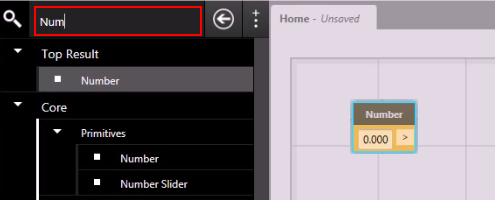
\includegraphics[width=0.8\textwidth]{img/dynam-tab}
   	\end{center}
   	\vspace{-15pt}
    \caption{Dynamo search tab.}
  \label{fig:dynam}
\end{figure}
\fi

\begin{wrapfigure}{r}{0.6\textwidth}
  \vspace{-20pt}
  \begin{center}
    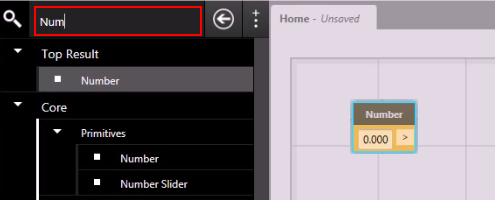
\includegraphics[width=0.6\textwidth]{img/dynam-tab}
  \end{center}
  \vspace{-15pt}
 \caption{Dynamo search tab. Searching for a component, highlighted in red.}  
  \vspace{-15pt}
    \label{fig:dynam}
\end{wrapfigure}

Dynamo provides a set of tools similar to Grasshopper, particularly it provides a searching table as shows Figure~\ref{fig:dynam}. This lateral table provides quick access to the primitives of the language, in this case the components. This feature encourages designers to explore the available components and try new components never ever tried.  

In general, Dynamo and Grasshopper are programming environments and visual languages popular among novices in programming. The smooth learn curve and perhaps the style of the \ac{ui} elements are attractive for beginners. However as the visual programs become large and complex it requires more time to understand, maintain, and adapt to new requirements, than the textual programs as showed in~\cite{leitao2011programming}. Despite of spending more time and effort to learn a textual programming language, the learners have their time quickly recovered once the complexity of the design task becomes sufficiently large.
%%%%%%%%%%%%%%%%%%%%%%%%%%%%%%%%%%%%%%%%%%%%%%%%%%%%%%%%%%%%%%%%%%%%%%%%%%%%%%%%%%%%%%%%%%%%%%%%%%%%%%%%%
\subsubsection{Mathematica~\cite{wolfram1991mathematica}} is a language and environment built to support scientific calculation. It is widely used in the scientific community, specially by students, because it is an artificial language in which typical computations and programs are expressed in the shortest and clearest possible way. For this, Mathematica supports not just liner textual input, but also full two-dimensional input, like traditional mathematical notation, as shows Figure~\ref{fig:math}.

\begin{wrapfigure}{r}{0.6\textwidth}
  \vspace{-20pt}
  \begin{center}
    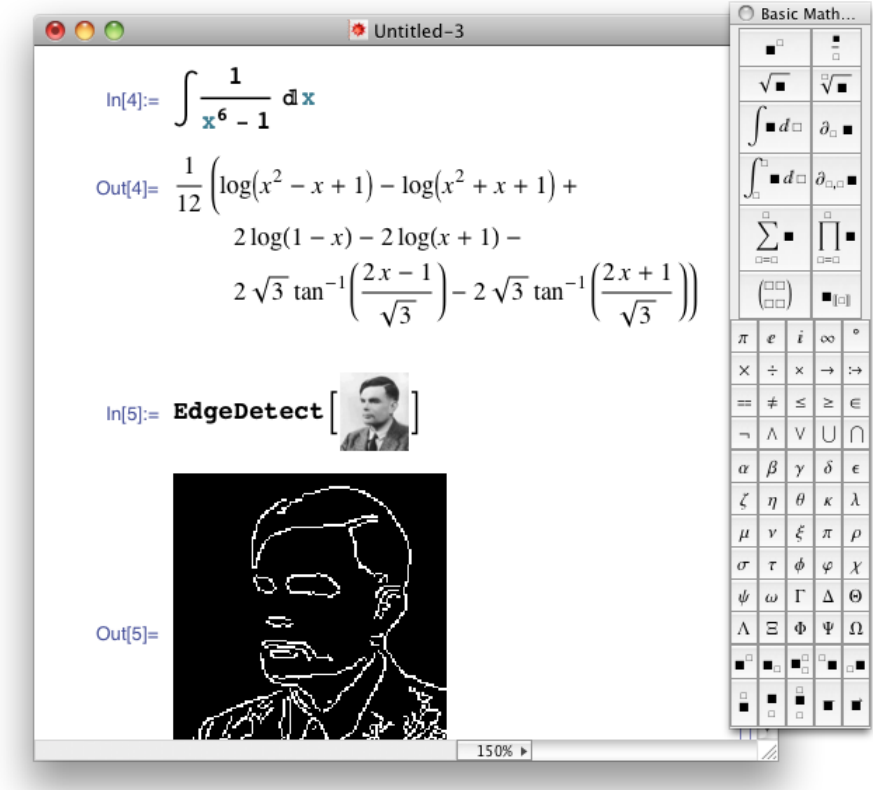
\includegraphics[width=0.6\textwidth]{img/mathematica}
  \end{center}
  \vspace{-15pt}
 \caption{Mathematica program. Note the two-dimensional character of the input.}  
  \vspace{-20pt}
    \label{fig:math}
\end{wrapfigure}

The core concept of Mathematica as such a language was based in the paradigm initiated by Turing's work~\cite{wolfram2003wolfram}. In this paradigm mathematical processes are systematized as computations. As a result, Mathematica represents mathematics by finding what is true explicitly computing output from input. 

Mathematica can internally represent any possible computation. The challenge it addresses is to connect those possible computations to ones that human can describe. Surprisingly to achieve this, it took only a modest set of innovations. Because there was a certain degree of consistency in the notation that people tended to use. In this way the main process basically is to convert this notation to something completely precise and computable. 

Present the information in a human readable format is undoubtedly a successful strategy of Mathematica's features. However the growing complexity of these features may overwhelm novices. Consequently, Mathematica is avoid in many subjects because it adds an extra complexity in a subject that is already quite difficult. On the other hand some mathematicians, and some students, seem to get so fascinated with the tools that the mathematics ends up relegated to a supporting role.
%%%%%%%%%%%%%%%%%%%%%%%%%%%%%%%%%%%%%%%%%%%%%%%%%%%%%%%%%%%%%%%%%%%%%%%%%%%%%%%%%%%%%%%%%%%%%%%%%%%%%%%%%
\subsubsection{IPython~\cite{PER-GRA:2007}} is a programming environment built to support scientific calculation. Originally, IPython was designed to be a mini Mathematica~\cite{wolfram1991mathematica}. Nowadays it supports a set of languages (frontends) and provides, among other features, an interactive shell and a browser-based notebook with support for code, text, mathematical expressions, plots and other rich media. 

IPython is implemented in Python to get access to the several libraries of math computation. Like Mathematica, a program in IPython explicitly computes an output from input. It is a useful paradigm for developing iteratively, because a program can be written in parts and each part is tested individually. However, IPython is focused on interoperability rather than present its computations to ones that humans can describe.

\begin{wrapfigure}{r}{0.6\textwidth}
  \vspace{-35pt}
  \begin{center}
    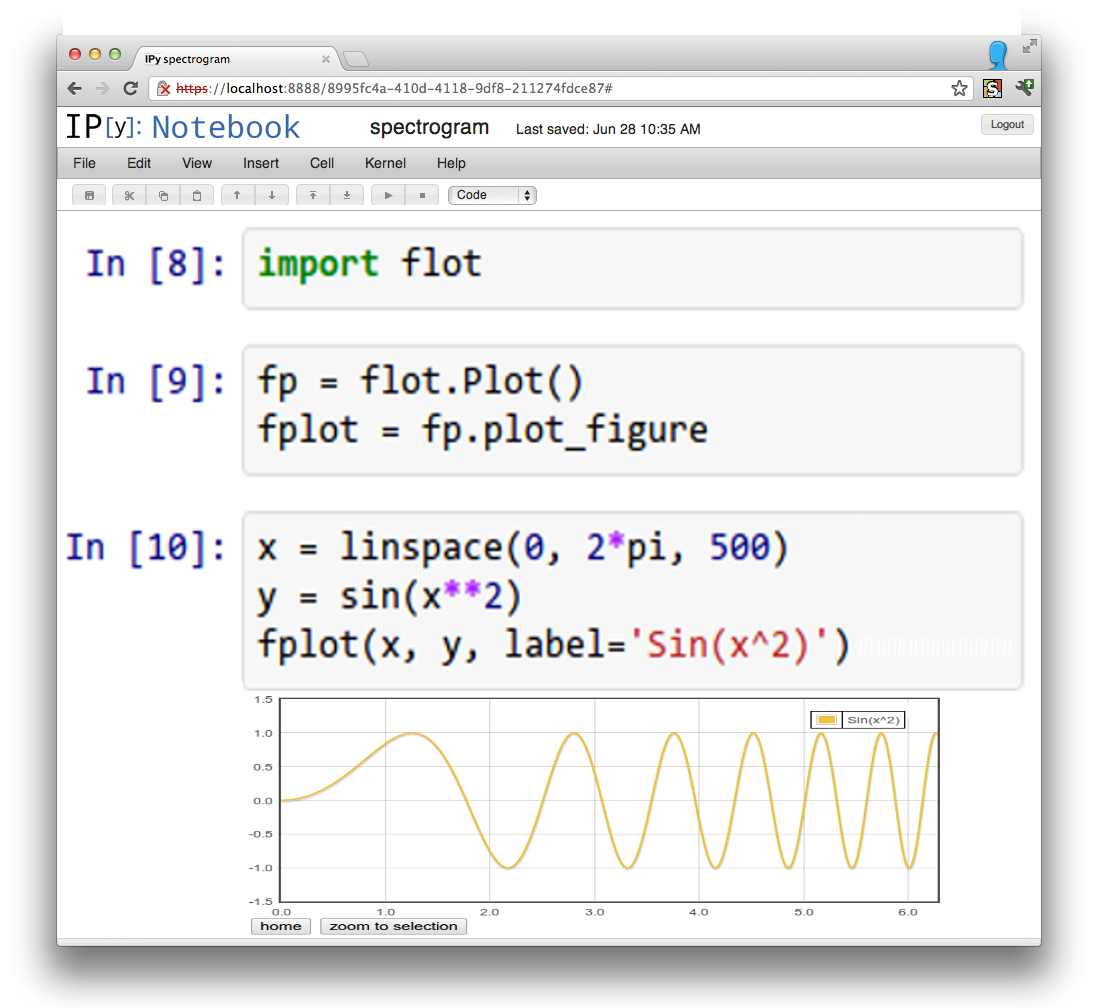
\includegraphics[width=0.6\textwidth]{img/ipython-zoom}
  \end{center}
  \vspace{-15pt}
 \caption{IPython browser-based notebook. The input is just linear characters.}  
  \vspace{-15pt}
    \label{fig:ipython}
\end{wrapfigure}

Figure~\ref{fig:ipython}, shows some interactions with the IPython notebook using Python language through a web browser. The IPython's architecture is a kind of client-server. The frontend language is the server and the notebook is the client. To support several frontends IPython provides a base layer for new programming environments. This layer exposes the major components of IPytohn's architecture. Consequently, IPython's features are available form others systems. For example, IJulia uses IPython interface with Julia language. 
%%%%%%%%%%%%%%%%%%%%%%%%%%%%%%%%%%%%%%%%%%%%%%%%%%%%%%%%%%%%%%%%%%%%%%%%%%%%%%%%%%%%%%%%%%%%%%%%%%%%%%%%%
\subsubsection{MathCAD\protect\footnote{\texttt{http://www.ptc.com/product/mathcad}}} is a programming environment and language built to support scientific calculation. Like Mathematica, MathCAD aims to present information into a human readable form. However, it generates live calculations with plots, graphs, text and images into a single document. This document is the program's environment as well as the final product.

The mathematical expressions defined in the MathCAD document act as an associative language. So when a expressions is changed its value is propagated through the document. This mechanism is the base of the interactiveness. However, as stated above, it represents an barrier for recomposition. Because new expressions can change the previous. Moreover, the MathCAD language is purely visual so it presents the same drawbacks identified above.
%%%%%%%%%%%%%%%%%%%%%%%%%%%%%%%%%%%%%%%%%%%%%%%%%%%%%%%%%%%%%%%%%%%%%%%%%%%%%%%%%%%%%%%%%%%%%%%%%%%%%%%%%		     

%%
\subsection{Summary}

Table~\ref{tab:sum} attempts to show the presented systems based on their major design influences. The table is also intended to address the following questions.

\begin{table}[h]
\centering
\resizebox{\textwidth}{!}{%
\begin{tabular}{@{}clllll@{}}
\toprule
\multicolumn{1}{l}{\textbf{Type$^{(1)}$}} & \textbf{System} & \textbf{Main feature}$^{(2)}$ & \textbf{\begin{tabular}[c]{@{}l@{}}Support to under-\\ stand programs$^{(3)}$\end{tabular}} & \textbf{\begin{tabular}[c]{@{}l@{}}Representation \\ of code$^{(4)}$\end{tabular}} & \textbf{\begin{tabular}[c]{@{}l@{}}Construction\\ of programs$^{(5)}$\end{tabular}} \\ \midrule
\multirow{6}{*}{GS} & Eclipse & \multirow{4}{*}{\begin{tabular}[c]{@{}l@{}}support software\\ development \\ life cycle\end{tabular}} & \multirow{4}{*}{debugger} & \multirow{16}{*}{text} & \multirow{16}{*}{typing code} \\
 & NetBeans &  &  &  &  \\
 & IntelliJ &  &  &  &  \\
 & MVS &  &  &  &  \\ \cmidrule(lr){2-4}
 & Xcode & \multirow{2}{*}{\begin{tabular}[c]{@{}l@{}}observable \\ programming\end{tabular}} & \multirow{2}{*}{\begin{tabular}[c]{@{}l@{}}live execution\\ feedback\end{tabular}} &  &  \\
 & LightTable &  &  &  &  \\ \cmidrule(r){1-4}
\multirow{7}{*}{TS} & LOGO & \multirow{2}{*}{\begin{tabular}[c]{@{}l@{}}understandable\\ language\end{tabular}} & \multirow{2}{*}{physical interpretation} &  &  \\
 & SmallTalk &  &  &  &  \\ \cmidrule(lr){2-4}
 & Processing & \multirow{2}{*}{visual context} & \multirow{2}{*}{instant visualization} &  &  \\
 & Fluxus &  &  &  &  \\ \cmidrule(lr){2-4}
 & DrRacket & gradual learning & debugger; stepper &  &  \\ \cmidrule(lr){2-4}
 & PythonTutor & \multirow{2}{*}{show program flow} & \multirow{2}{*}{\begin{tabular}[c]{@{}l@{}}navigate through the \\ program execution\end{tabular}} &  &  \\
 & YinYang &  &  &  &  \\ \cmidrule(r){1-4}
\multirow{8}{*}{ES} & DesignScript & \multirow{3}{*}{\begin{tabular}[c]{@{}l@{}}support\\ generative\\ design methods\end{tabular}} & \multirow{3}{*}{debugger} &  &  \\
 & Monkey &  &  &  &  \\
 & Rosetta &  &  &  &  \\ \cmidrule(l){2-6} 
 & Grasshopper & \multirow{2}{*}{\begin{tabular}[c]{@{}l@{}}alternative way to \\ expressing programs\end{tabular}} & \multirow{2}{*}{dataflow paradigm} & \multirow{2}{*}{\begin{tabular}[c]{@{}l@{}}graphical \\ components\end{tabular}} & \multirow{2}{*}{\begin{tabular}[c]{@{}l@{}}linking\\ components\end{tabular}} \\
 & Dynamo &  &  &  &  \\ \cmidrule(l){2-6} 
 & Mathematica & \multirow{3}{*}{\begin{tabular}[c]{@{}l@{}}support \\ scientific calculation\end{tabular}} & \multirow{3}{*}{\begin{tabular}[c]{@{}l@{}}present data \\ meaningfully\end{tabular}} & \multirow{3}{*}{\begin{tabular}[c]{@{}l@{}}mathematical\\ forms\end{tabular}} & \multirow{3}{*}{fill forms} \\
 & IPython &  &  &  &  \\
 & MathCAD &  &  &  &  \\ \bottomrule
\end{tabular}
}
\caption{System Attributes.}
\label{tab:sum}
\end{table}


(1) \textit{What is the purpose of the system?} We categorized three main purposes which a system can be designed. \ac{gs} designed for building complex software for the industry. \ac{ts} designed to help people learn to program. \ac{es} designed to allow people build things that are tailored to their own needs.

(2) \textit{How does the system support its purpose?} We identified the following strategies. (i) Support software development life cycle, (ii) make programming in something observable, (iii) create an understandable language, (iv) combine textual programming with a visual context, (v) support gradual learning in a single environment, (vi) show the program flow, (vii) support generative design methods, (viii) find alternative ways to typing programs and (ix) support scientific calculation.

(3) \textit{Does the programming environment provide additional support to enable users to better understand the behavior of their programs?} Environments in our study used several techniques to help users understand the behavior of their programs. These included (i) a debugger that stops the program execution allowing users to inspect line-by-line (ii) live execution feedback (iii) physical interpretation (iv) instant visualization (v) navigate through the program execution (vi) dataflow paradigm and (vii) present data as humans understand.

(4) \textit{How does code look in the programming environment or language?} The systems in our study represent programs using text, graphical components, users can manipulate, and mathematical forms users can fill in.

(5) \textit{What actions do users take to construct programs?} Users can construct programs by typing code, linking graphical components and editing mathematical forms.